\section{Bildebehandling}
Gir en verktøykasse for analyse av et bilde. Du kan dele opp i tre nivåer:
\begin{itemize}
    \item High-level. Computer vision.
    \item Mid-level. Image understanding, segmentering.
    \item Low-level. Noise reduction og andre ting som får bildet bedre for prosessering.
\end{itemize}
\subsection{Typical Image Processing Steps}
Dette har vært spørsmål på flere eksamenssett.
\subsubsection{Image acquisition}
\begin{itemize}
    \item Få inn et digitalt bilde.
    \item Recording.
    \item Sampling.
    \item Skalering.
\end{itemize}

\subsubsection{Image Enchancement}
Subjektiv prosess for å få bildet til å se bedre ut. Målet er å gjøre bildet passende for det det skal brukes til.

\subsubsection{Image Restoration}
Målet er å bruke matematiske modeller for å gjøre bildet bedre (feks fjerne støy).

\subsubsection{Morphological Processing}
Hente ut bildekomponenter, gjerne lage binære bilder.

\subsubsection{Segmentation}
Partisjonere bildet inn i meningsfulle biter, gjerne forgrunn/bakgrunn.

\subsubsection{Representation and description}
Ta ut attributter for å skille objekter fra hverandre.

\subsubsection{Object Recognition}
Finne ut hva et objekt er (er det en bil?)

\subsection{Menneskeøyet}
Består av to forskjellige "receptor classes", cones (6-7 millioner, fargesyn, hver har sin nervetråd) og rods (75-150 millioner, sensitive for lavt lys, flere kan være knyttet til en enkelt nervetråd)
\\ 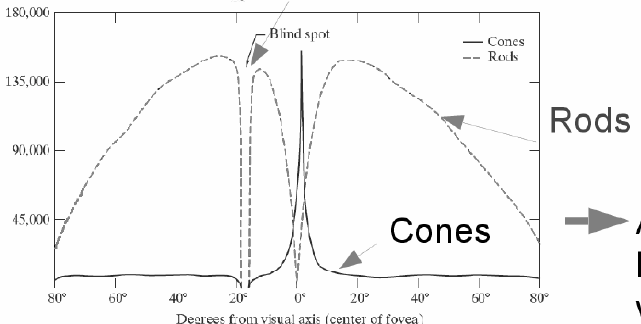
\includegraphics[width=\textwidth]{Bilder/rodscones.png}
Den blinde flekken er en nervetråd som kommer ut (feil fra evolusjonen) som gjør at det ikke er noen cones eller rods på et lite område.

\subsection{Sampling}
Gjøre om fra analogt til digitalt. 

De sier at sampling: discretization of a signal (spatial or temporal) og quantization: assign a discrete intensity value to the signal. Med andre ord; sampling er å skanne med diskrete koordinater (tid og rom), quantization er å gjøre om disse samplene til diskrete verdier.

Nyquist-Shannon sampling theorem sier at:
\begin{equation}
    f_s > 2 f_{max}
\end{equation}
Samplefrekvensen må minst være dobbelt så stor som den høyeste frekvensen man finner i bildet. Vi foretrekker blur foran aliasing-effekter, så kjør over med et lavpassfilter før man skalerer ned et bilde.

\subsection{Image Sensing and Acquisition}
Et kamera har en matrise med sensorer. For å få farger på disse, legger man på fargefiltre over hver sensor, gjerne to grønne per blå og rød, siden øyet vårt er mer sensitivt for grønn-farger. Vi kan gå fra RGB til grayscale med denne formelen:
\begin{equation}
    luminance = 0.30R + 0.59G + 0.11B
\end{equation}
\subsection{Naboskap}
De to vanligste formene for naboskap er 4-nabo (kryss) eller 8-nabo (3x3-kvadrat med ramme). Vi har også avstandsfunksjoner:

City block:
\begin{equation}
D_4(p,q) = |x_p - x_q| + | y_p - y_q |
\end{equation}
Chess-board:
\begin{equation}
D_8(p,q) = max(|x_p - x_q|, |y_p - y_q|)
\end{equation}
Euclidian:
\begin{equation}
D_E(p,q) = \sqrt{|x_p - x_q|^2 + |y_p - y_q|^2}
\end{equation}

\subsection{Spatial image enhancement}
En operasjon i spatial domain blir uttrykt på følgende måte:
\begin{equation}
    g(x,y) = T[f(x,y)]
\end{equation}
der $f(x,y)$ er input image og T er en operasjon definert på nabolaget til $(x,y)$. Hvis nabolaget bare består av en piksel, snakker vi om en \emph{intensity transformation} eller en \emph{point processing operation}:
\begin{equation}
    q = T(p)
\end{equation}
Dette brukes til kontrastmanipulering og image thresholding.

\subsection{Negativt bilde}
\begin{equation}
T(p) = 255-p
\end{equation}

\subsection{Logarithmic Transform}
\begin{equation}
    q = T(p) = c*log(1+p)
\end{equation}
Denne kan komprimere den dynamiske rekkevidden til et bilde.

\subsection{Gamma Transformations}
Veldig allsidig transformasjon for å utvide enten mørke eller lyse områder i et bilde.
\begin{equation}
    q = cp^\gamma, c > 0, \gamma > 0
\end{equation}
$\gamma < 1$ Utvider lave intensiteter, $\gamma > 1$ utvider høye intensiteter. Kan hjelpe til å vise bilder bedre på skjermer ved å gamma-justere bildene før visning.

\subsection{Histogrammet til et bilde}
Et histogram til et bilde gir informasjon om spredningen av intensitetsverdiene. En funksjon $h(k)$ teller antall piksler med verdi $k$.
\begin{equation}
    h(k) = \sum_{(ij) \in  \Omega} \delta (I_{ij} - k)
\end{equation}
der $\delta$ er 1 dersom $x=0$. man kan normalisere et histogram ved å dividere på antall piksler:
\begin{equation}
    p(k) = {h(k) \over MN}
\end{equation}

\subsubsection{Mean and Variance}
Vi kan bruke histogrammet til å regne ut forventningsverdi og varians dersom vi allerede har et normalisert histogram, $p(k)$.

\begin{equation}
    m = \sum_{k=0}^{L-1} k p(k)
\end{equation}
\begin{equation}
    \sigma^2 = \sum_{k=0}^{L-1} (k-m)^2 p(k)
\end{equation}

\subsection{Histogram Equalization}
Vi ønsker oss en \emph{intensity transform}-funksjon som sprer ut histogrammet vårt. Det viser seg at en skalert versjon av den kumulative intensitetsdistribusjonen gjør nytten.
\begin{enumerate}
    \item Regn ut den kumulative fordelingen av grå-verdier. Siste verdi her skal tilsvare antall piksler i bildet (NM).
    \item Normaliser, altså divider med antall piksler i bildet (NM).
    \item Multipliser med antall gråverdier du har i bildet, og rund disse verdiene av til nærmeste heltall.
    \item Siste rad (i punktet ovenfor) utgjør nå en mapping fra gamle til nye gråverdier.
\end{enumerate}

\subsubsection{Histogram Equalization med farger}
Hvis man kjører HE-algoritmen på fargene enkeltvis, vil fargene bli forskjøvet. En vanlig metode er å kjøre en kombinert HE på intensitet og saturation i HSI-fargemodellen

\subsection{Støytyper}
\begin{itemize}
    \item Normal (Gaussian) noise. Vanlig type støy, hvor støyen per piksel er uavhengig av intensiteten på signalet.
    \item Uniform noise. Likt fordelt utover et gitt intervall [a,m]
    \item Salt-and-pepper noise. Svarte og hvite piksler, kan forekomme av overføringsfeil og lignende.
    \item Annet: Exponential, poisson, speckle noise, ayleight, gamma...
\end{itemize}

\subsection{Bit plane slicing}
Høyere bits er mer viktige enn lavere bits.
\\ 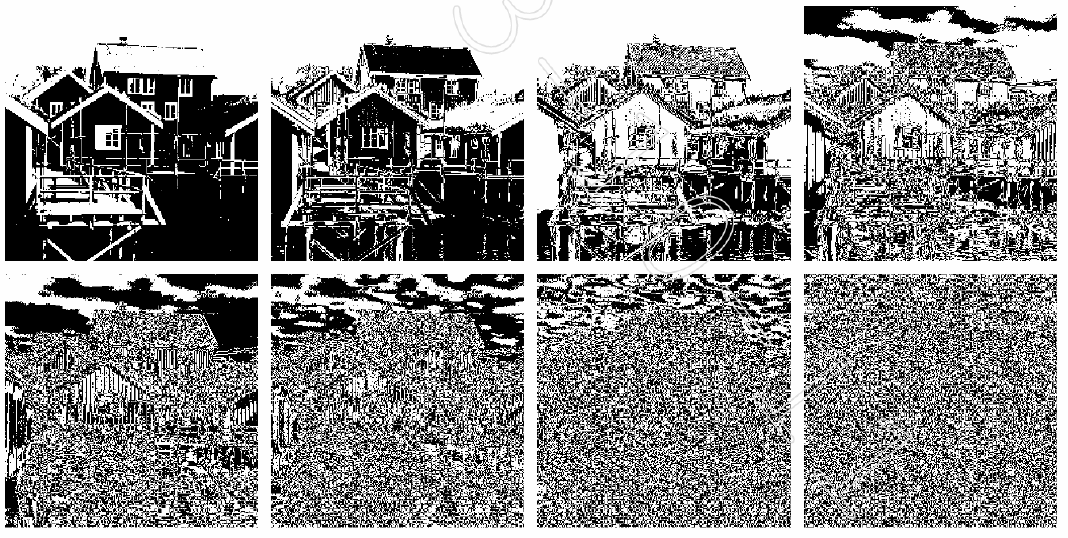
\includegraphics[width=\textwidth]{Bilder/bitplaneslicing.png}

\subsection{Neighborhood Processing}
Beskrevet flott slik:
\begin{enumerate}
    \item Definér et senterpunkt.
    \item Gjør en operasjon på pikslene i nabolaget.
    \item La responsen herifra bestemme verdien på valgt senterpiksel.
    \item Rinse repeat på resten av pikslene i bildet.
\end{enumerate}
De fleste filtre er av odde størrelse, slik at naboene blir vektlagt likt.

\subsubsection{Lineære filtre}
Dersom et filter representerer en lineær kombinasjon av intensitetene til nabolaget kan det kalles lineært.
\begin{equation}
    g_{i,j} = \sum_{s=-a}^a \sum_{t=-b}^b w_{s,t} x_{x+s, j+t}
\end{equation}

\subsection{Average/box filter}
Normalisert matrise med like elementer og summen er 1.0. Følge av at summen er 1.0, er at gjennomsnittlig gråverdi ikke er endret.

\subsection{Korrelasjon og konvolusjon}
Korrelasjon:
\begin{equation}
    g_{i,j} = \sum_{s=-a}^a \sum_{t=-b}^b w_{s,t} x_{x+s, j+t}
\end{equation}
Konvolusjon:
\begin{equation}
    g_{i,j} = \sum_{s=-a}^a \sum_{t=-b}^b w_{s,t} x_{x-s, j-t}
\end{equation}
Sistnevnte ble introdusert for å la en enhetsrespons bli lik filteret. For å utføre en konvolusjon, må du snu masken 180 grader. Hvis filteret er symmetrisk er korrelasjon og konvolusjon det samme. Konvolusjon er lineært.

\subsection{Padding}
Padding skjer når man ønsker å utvide kantene på et bilde (for eksempel hvis man skal kjøre et spatial filter). Vi har fire typer:
    \begin{itemize}
        \item Zero/Constant padding. Fyll inn resten av bildet med null eller gjennomsnittlig farge/gråverdi.
        \item Symmetric/Reflection padding. Reflekter kanten. Symmetrisk gjentar du alle pikslene i motsatt rekkefølge (2 1 0 | 0 1 2), med reflection hopper du over første piksel (2 1 0 1 2).
        \item Replicate padding. Kopiér pikselen som var på kanten.
        \item Circular padding. Gjenta bildet.
    \end{itemize}
    
\subsection{Smoothing}
Man kan smoothe med både lineære og ikke-lineære filtre. Et eksempel er \emph{Average/box filter}. Man kan også bruke vektet gjennomsnittsverdi:
\begin{equation}
    {1 \over 16} \times \begin{bmatrix}
        1 & 2 & 1 \\
        2 & 4 & 2 \\
        1 & 2 & 1
    \end{bmatrix}
\end{equation}

Et godt ikke-lineært filter for salt-and-pepper noise er median filtering, der man finner medianen til nabolaget.

\subsection{Derivasjonsfiltre}
Et godt filter for den deriverte er $\begin{bmatrix} -1 & 1 \end{bmatrix}$. Et godt filter for den andrederiverte er $\begin{bmatrix} 1 & -2 & 1 \end{bmatrix}$.

Vi har også laplacian:
\begin{equation}
    \begin{bmatrix}
        0 & 1 & 0 \\
        1 & -4 & 1 \\
        0 & 1 & 0
    \end{bmatrix}
\end{equation}
Med denne får du både positive og negative verdier.

Dette filteret kan vi bruke til å forsterke kanter i et bilde
\begin{equation}
    Original - Laplacian filtered = Sharpened
\end{equation}
Hvorfor fungerer dette? LaPlace er den andrederiverte til et bilde, og ved å trekke fra resultatet her, vil du få forsterkede kanter (fordi den andrederiverte er sterkest der frekvensene endrer seg fortest. Se \ref{subsection:unsharp_mask}

En raskere måte å gjøre dette på er å ta det motsatte av laplacian og øke fra 4 til 5 i senterelementet. Bruk det da som et vanlig spatial filter, siden summen av elementene er 1.

\subsection{Sharpening by Unsharp Mask}\label{subsection:unsharp_mask}
Dette bildet forklarer det meste:
\\ 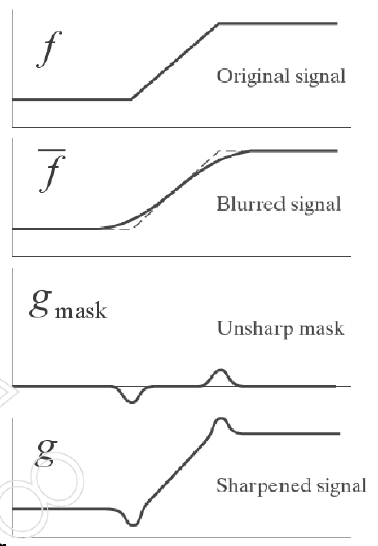
\includegraphics[width=\textwidth]{Bilder/unsharp_mask.png}
Når man adderer $g_{mask}$ etterpå, kan man gjøre dette med en faktor $k$ for å få \emph{highboost}.

\subsection{Filtre for deriverte}
Roberts (for skrå gradienter):
\begin{equation}
    \begin{bmatrix}
        -1 & 0 \\
        0 & 1
    \end{bmatrix}
\end{equation}
\begin{equation}
    \begin{bmatrix}
        0 & -1 \\
        1 & 0
    \end{bmatrix}
\end{equation}
Sobel (siden vi foretrekker filtre av odde størrelse):
\begin{equation}
    \begin{bmatrix}
        -1 & 0 & 1 \\
        -2 & 0 & 2 \\
        -1 & 0 & 1
    \end{bmatrix}
\end{equation}
\begin{equation}
    \begin{bmatrix}
        -1 & -2 & -1 \\
        0 & 0 & 0 \\
        1 & 2 & 1
    \end{bmatrix}
\end{equation}

\subsubsection{Gradient}
Siden vi operer med deriverte i både x- og y-retning, er en absoluttverdi fint å ha. Dette bildet heter gradient eller gradientbilde.
\begin{equation}
    |\nabla f| = \sqrt{
        ({\partial f \over \partial x})^2 + ({\partial f \over \partial y})^2
    }
\end{equation}
Kan approksimeres ved å summere sammen absoluttverdi for x- og y-derivert.

\subsection{1.- og 2.-deriverte}
1.-deriverte vil resultere i tykkere kanter, får respons i "oppoverbakker". Sterk respons på grånivåsteg. 2.-deriverte vil gi større respons til detalj, og få zero crossing ved grånivåsteg.
\subsection{Gaussian}
For 1-dimensjon gjelder:
\begin{equation}
    N(x, \sigma) = {1 \over \sigma\sqrt{2\pi}}\mathrm{e}^{-x^{2} \over 2\sigma}
\end{equation}

For to dimensjoner er det bare å multiplisere disse uttrykkene sammen:
\begin{equation}
    N(x, \sigma) = {1 \over \sigma^{2}2\pi}\mathrm{e}^{-({x^{2} + y^2}) \over 2\sigma}
\end{equation}

En god approksimasjon er binomialkoeffesientene.

En direkte konsekvens av at gaussian er separabel, er at vi kan gjøre 1-dimensjonal filtering i x- og y-retning. Vi kan med andre ord gjøre en konvolusjon mellom to 1-dimensjonale gauss-filtre for å få et som fungerer for 2D.

De sier at Gaussian er den mest sentrale smoothe-operatoren i bildebehandling. Smoothing er uavhengig av bilderotasjon.

\subsubsection{Gaussian i frekvensdomenet}
Fouriertransformen til en Gaussian med standardavvik $\sigma$ er er annen Gauss med standardavvik proposjonal med ${1 \over \sigma}$

\subsection{Conservative smoothing}
Denne algoritmen sjekker hele nabolaget (utenom referansepikselen) og finner $min$ og $max$ her. Dersom referansepikselen ikke er i dette intervallet, sett den til $min$ eller $max$, avhengig av hva som er nærmest. Dette er et ikke-lineært filter.

\subsection{Smoothing and Derivative filters}
\begin{center}
    \begin{tabular}{| p{5cm} | p{5cm} |}
        \hline
            (Linear) Smoothing Filters & Derivative/Gradient Filters \\ 
        \hline
            Mål: Fjerne støy og små endringer i bildet. & Mål: Finne områder i bildet med raske endringer (kanter). \\
        \hline
            Normalisert til 1.0 & Sum er 0.0 \\
        \hline
            Ingen endring i grå-verdi i homogene områder. & Nullrespons i homogene områder. \\
        \hline
            I frekvensdomenet: Fjerne høye frekvenser (low-pass filter). & I frekvensdomenet: Fjerne lave frekvenser (high-pass filter).\\
        \hline
            Ulempe: Jevner ut ønskede detaljer (som kanter) & Ulempe: Blir mer støy \\
        \hline
    \end{tabular}
\end{center}

\subsection{Fouriertransformasjon}
Fouriers idé var at alle periodiske funksjoner kunne bli representert som en vektet sum av sinuser og cosinuser.
Den todimensjonale diskrete fouriertransformasjonen til et bilde $f(x,y)$ av størrelse MxN er:
\begin{equation}
    F(u,v) = \sum_{x=0}^{M-1}\sum_{y=0}^{N-1} f(x,y) e^{
        -2\pi i( {ux \over M} + {vy \over N} )
    }
\end{equation}
Den inverse diskrtere fouriertransformasjonen er:
\begin{equation}
    f(x,y) = {1 \over NM}\sum_{x=0}^{M-1}\sum_{y=0}^{N-1} F(u,v) e^{
        2\pi i( {ux \over M} + {vy \over N} )
    }
\end{equation}
Forutsetninger:
\begin{itemize}
    \item f(x,y) kan være en kompleks funksjon (ha både reell og imaginær del).
    \item f(x,y) må være periodisk i x med periode N og i y med periode M.
\end{itemize}

\subsubsection{Visualisering}
Vi kan representerer et kompleks nummer $c = a+ib$ med amplitude $\sqrt{Re^2(c)+Im^2(c)}$ og fase $\Theta = atan2(Im(c), Re(c)$. Et kompleks nummer er da på formen:
\begin{equation}
    c = r e^{i\Theta}
\end{equation}
Per piksel $(u,v)$ i et bilde kan man vise både amplitude og fase i et NxM-bilde.

Siden fouriertransformen får negative- og positive verdier, samt en reel og en imaginær del, kan vi regne ut amplituden slik som dette:
\begin{equation}
    |F(u,v)| = \sqrt{Re^2(F(u,v)) + Im^2(F(u,v))}
\end{equation}

Siden $F(0,0)$ er senter av spekterbildet, kan det lønne seg å shifte bildet med $({M \over 2},{N \over 2})$. Man kan også multiplisere bildet med et \emph{chess board pattern} før man tar bildet over i frekvensdomenet. 

\subsubsection{Kjøretid}
Siden vanlig fouriertransform er $O(N^2)$, har man funnet på en effektiv \emph{Fast Fourier Transform} med kjøretid $O(N log_2(N))$. Fouriertransformen er separabel, så man kan kjøre den først i x-retning, så i y-retning.

\subsubsection{Annet}
\begin{equation}
    F(u,v) = F*(-u, -v)
\end{equation}
Dette medfører at spektrumet viser symmetri om origo i en visualisering.

\subsubsection{Skalering}
\begin{equation}
    \mathscr{F} \left\{f(\alpha x)\right\} = {1 \over |\alpha|}F({u \over \alpha})
\end{equation}


\subsubsection{Convolution og Fourier}
\begin{equation}
    f \ast g = \mathscr{F}^-1 \left\{\mathscr{F}\left\{f\right\} \cdot \mathscr{F}\left\{g\right\}\right\}
\end{equation}
Dette betyr at en konvolusjon i spatial domain er det samme som en multiplikasjon (pikselvis) i frequency domain. For å gjøre om et spatial filter, må man padde med sort-verdier og kjøre fouriertransform.

\subsection{Frequency Filter Interpretation}
Vi kan få ut informasjon fra et bilde visualisert i frekvensdomenet:
\\ 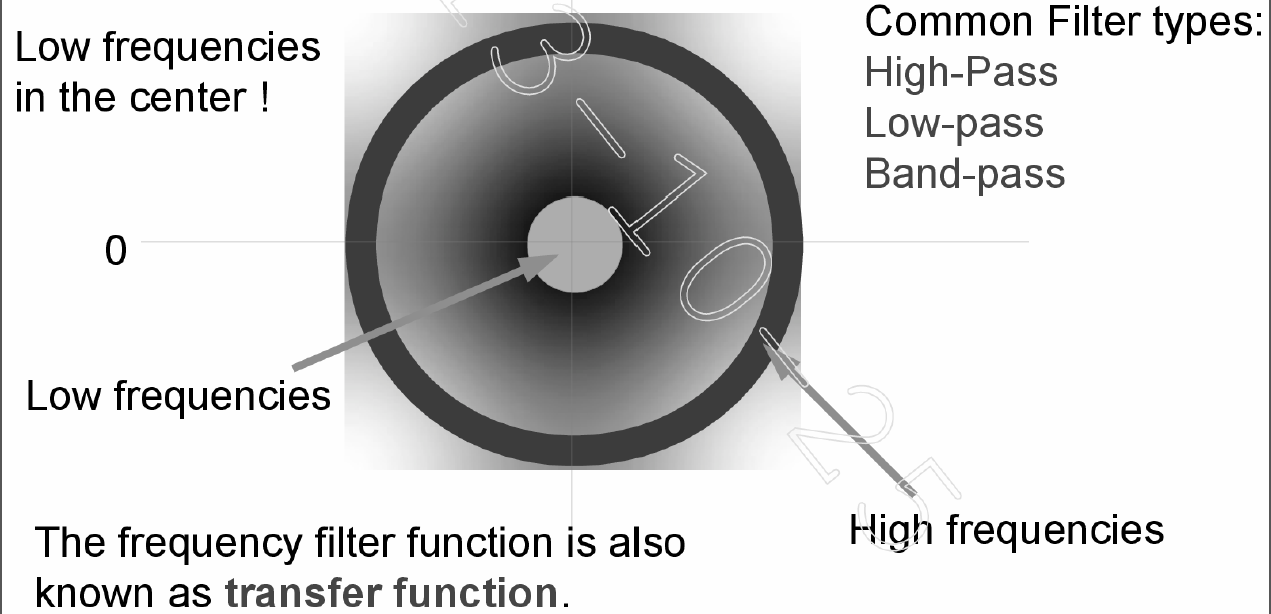
\includegraphics[width=\textwidth]{Bilder/ffi.png}

\subsection{Ideelt lav-passfilter}
\begin{equation}
    H(u,v) = \left\{
        \begin{array} {ll}
            1 & \quad \text{if $D(u,v) \le D_0$} \\
            0 & \quad \text{if $D(u,v) > D_0$}
        \end{array}
        \right.
\end{equation}
$D_0$ er cutoff. Dette vil gi ringing effects, siden boks-funksjonen er en \emph{sinc-fuksjon} i spatial domain.
\\ 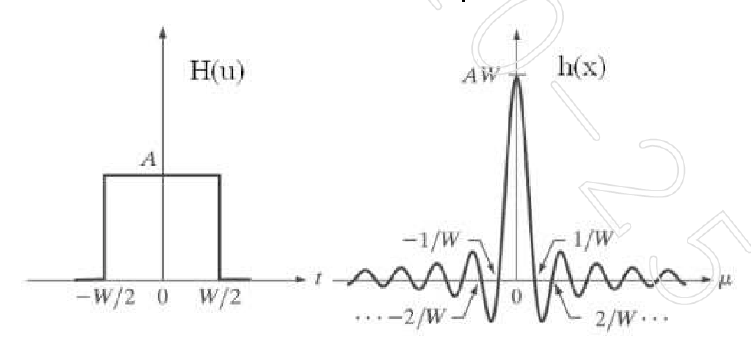
\includegraphics[width=\textwidth]{Bilder/ringing.png}

\subsection{Butterworth Low-pass Filter}
Siden et ideelt lavpassfilter lager "ringing effects", var det en smarting som lagde en jevnere funksjon.
\begin{equation}
    H(u,v) = {1 \over
        1 + ({D(u,v) \over D_0})^{2n}
    }
\end{equation}
Her er $D(u,v)$ distansen fra sentrum og $D_0$ cutoff-verdien. Jo høyere $n$, jo brattere bakke. $D_0$ representerer verdien der funksjonen er 0.5.

\subsection{Gaussian Low-pass filter}
\begin{equation}
    H(u,v) = e^{
        -D^2(u,v) \over
        2D_0^2
    }
\end{equation}
Her er $D(u,v)$ distansen fra sentrum og $D_0$ cutoff-verdien.

Det viser seg at en gauss i frekvensdomenet er en gauss i spatial domian.

\subsection{Hva kan vi bruke lav-pass-filtre til?}
Vi kan bruke det for å fjerne støy og fine detaljer i et bilde. Vi kan også slå sammen segmenter som ikke henger sammen (f.eks. en tekst) ved å blurre bildet.

\subsection{High-pass filtering}
Høy-pass-filtre slipper igjennom høye frekvenser. Generell formel, hvis man har lavpass:
\begin{equation}
    H_{HP}(u,v) = 1 - H_{LP}(u,v)
\end{equation}


\subsection{Butterworth high pass filter}
\begin{equation}
    H(u,v) = {1 \over
        1 + ({D_0 \over D(u,v)})^{2n}
    }
\end{equation}
\subsection{High-Frequency Emphasis Filtering}
Dersom man ikke vil kvitte seg fullstendig med lave frekvenser, ikke la et høy-passfilter gå helt "til bunns", men la det være igjen $k_1$, slik at lave frekvenser blir mindre fokuselt på, men likevel er tilstede.
\\ 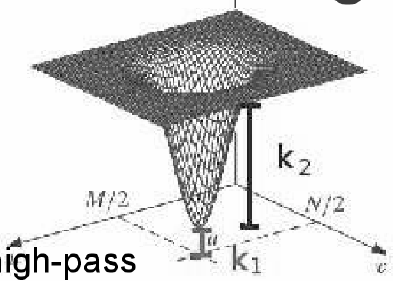
\includegraphics[width=\textwidth]{Bilder/hfef.png}
\begin{equation}
    G(u,v) = (k_1 + k_2*H_{HP}(u,v))*F(u,v)
\end{equation}

\subsection{Notch Filters}
Man kan ha store forekomster av gitte frekvenser i et bilde (periodisk støy). Disse vil være klare "prikker" i FD. En vanlig måte å representere et notch filter på er som et produkt av to høypass-filtre (gjerne gauss) i punktene $(u_k, v_k)$ og $(-u_k, -v_k)$.

\subsection{Segmentering}
Segmentering er en oppdeling av et bilde inn i flere regioner, og partisjonene skal tilsvare objekter i bildet.

To regioner er \emph{adjacent} når de har felles kant.

For gråtonebilder, pleier man å dele opp enten i similaritet eller diskontinuitet.

\subsection{Thresholding}
Dette er oppgaven å gjøre en binær beslutning om en verdi er over eller under en gitt verdi (terskel). Målet med operasjonen ifm. segmentering er å finne ut om en piksel er av interesse eller ikke.

Det finnes tre typer thresholding:
\begin{itemize}
    \item Global - T er brukt for hele bildet
    \item Variabel - T endres over et bilde
    \item Lokal/regional - T er avhengig av naboene til en piksel
\end{itemize}

\subsubsection{Bestemme T}
Dette er det viktigste punktet med en thresholdingalgoritme. T er gjerne i daler i histogrammet.
\\ 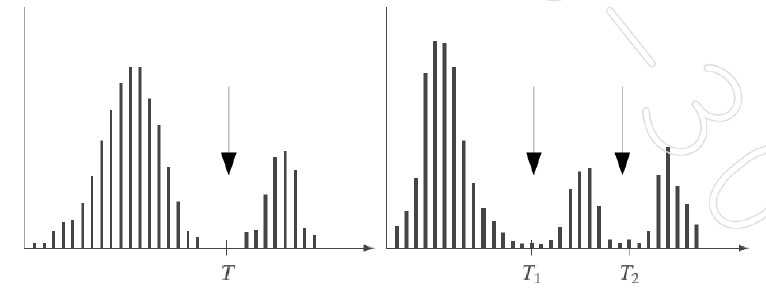
\includegraphics[width=\textwidth]{Bilder/thresholdhist.png}

Å finne en god T er avhengig av hvordan verdiene er spredt i histogrammet. Påvirket av:
\begin{itemize}
    \item Støy i bildet
    \item Relativ størrelse for objekter i forhold til bakgrunn.
    \item Jevn lyskilde.
    \item Jevn refleksjon i objekt/bakgrunn.
\end{itemize}

\paragraph{Basic global}
\begin{enumerate}
    \item T = gjennomsnittlig gråverdi for bildet
    \item Du får to sett, med $m_1$ og $m_2$ som gjennomsnittlig gråverdi for de to settene.
    \item Ny T = ${1 \over 2}(m_1 + m_2)$
    \item Hold på til endring i T per iterasjon blir liten nok
\end{enumerate}

\paragraph{Otsu}

Vanskelig å forklare, men prinsippet er sånn:

\begin{enumerate}
    \item Del opp i to deler.
    \item Regn ut varians i hver del.
    \item Målet er å få så liten varians som mulig i begge delene.
    \item Dette er det samme som å maksimerer variansen mellom de to delene (visstnok...)
\end{enumerate}

\begin{equation}
    \sigma^2(k) = P_1(k)[m_1(k)-m_G]^2 + P_2(k)[m_2(k)-m_G]^2
\end{equation}

Det blir enklest å normalisere histogrammet først (for videre utregninger):
\begin{equation}
    p_q = {n_q \over n}
\end{equation}

Andelene av piksler under og over k:
\begin{equation}
    P_1(k) = \sum_{i=0}^{k} p_i
\end{equation}
\begin{equation}
    P_2(k) = 1 - P_1(k)
\end{equation}
Snittverdier (forvetningsverdier, fra statistikk):
\begin{equation}
    m_G = \sum_{i=0}^{L-1}i p_i
\end{equation}
\begin{equation}
    m_1(k)= \sum_{i=0}^{k}i p_i
\end{equation}
\begin{equation}
    m_2(k)= \sum_{i={k+1}}^{L-1}i p_i
\end{equation}

Gå igjennom alle $k$-verdier og finn ut hva som gir høyeste verdi! \\
Otsus metode er optimal fordi den finner maks inter-klasse-varians mellom to klasser: Forgrunn og bakgrunn

\subsubsection{Variable Thresholding}
Enkleste er å dele opp bildet i flere deler og kjøre thresholding med algoritmene over på hvert enkelt histogram. Dette fungerer ikke når partisjonene inneholder kun bakgrunn- eller forgrunn.

Dersom man ønsker å utføre variabel thresholding, har man to muligheter. Den første er å vekte thresholdet etter standardavvik og forventningsverdi lokalt:
\begin{equation}
    T_{xy} = a\sigma_{xy} + b m_{xy}
\end{equation}
En annen er å bruke lokalt standardavvik, men global forventningsverdi:
\begin{equation}
    T_{xy} = a\sigma_{xy} + b m_{G}
\end{equation}
Man kan også bruke boolske operatorer

\subsubsection{Korreksjon av Shading Pattern}
\begin{itemize}
    \item Fikset belysning kan bli korrigert med å multiplisere av det inverse mønsteret av lyskilden (tatt opp på en flat, uniform overflate).
    \item Finne global belysning ved en \emph{top-hat transformation}.
    \item Bruk variabel eller lokal thresholding.
\end{itemize}

\subsubsection{Improving Global Thresholding}
Støy ødelegger alt. Hvis man smoother først, vil man få et histogram som er langt mer egnet for thresholding.

Dersom man kun skal finne en liten detalj, bruk et gradientfilter for å finne kant-piksler. La kun disse pikslene brukes til å lage histogrammet. Histogrammet du da får er egnet til å thresholde med, bruk feks otsus metode.

\subsection{Point Detection}
Man kan ofte finne punkter med følgende filter:
\begin{equation}
    \begin{bmatrix}
        -1 & -1 & -1 \\
        -1 & 8 & -1 \\
        -1 & -1 & -1
    \end{bmatrix}
\end{equation}
Denne er uavhengig av retning, og responderer til en enkel diskontinuitet i grå-verdi.

Man kan kjøre over dette filteret (laplace) og etterpå kjøre thresholding for å finne diskontinuiteter som er "store nok".

\subsection{Line detection}
Man kan bruke Laplacian for linjer også. Denne gir positive- og negative verdier. Hvis du tar absoluttverdien av dette, får du ganske tykke kanter. Hvis du bare bruker én av dem, får du tynnere kanter.
Se figur:
\\ 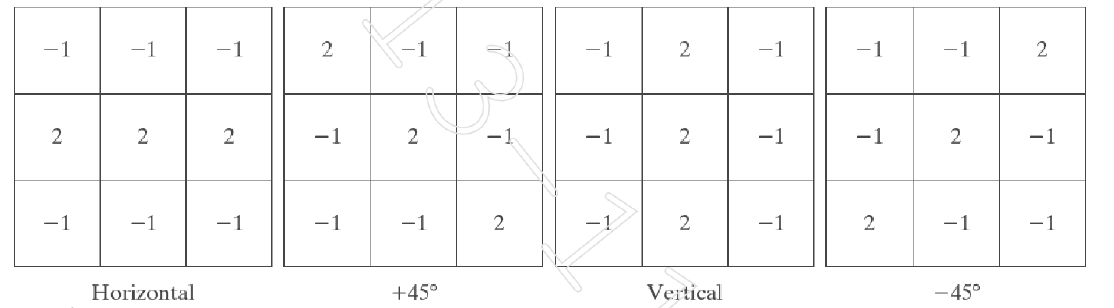
\includegraphics[width=\textwidth]{Bilder/line_detection.png}

Hvis man bruker alle maskene samtidig, kan den med størst respons brukes.

\subsection{Edge detection}
Blir noe annet enn line detection, her holder det med første-deriverte. Vanlige masker:
\\ 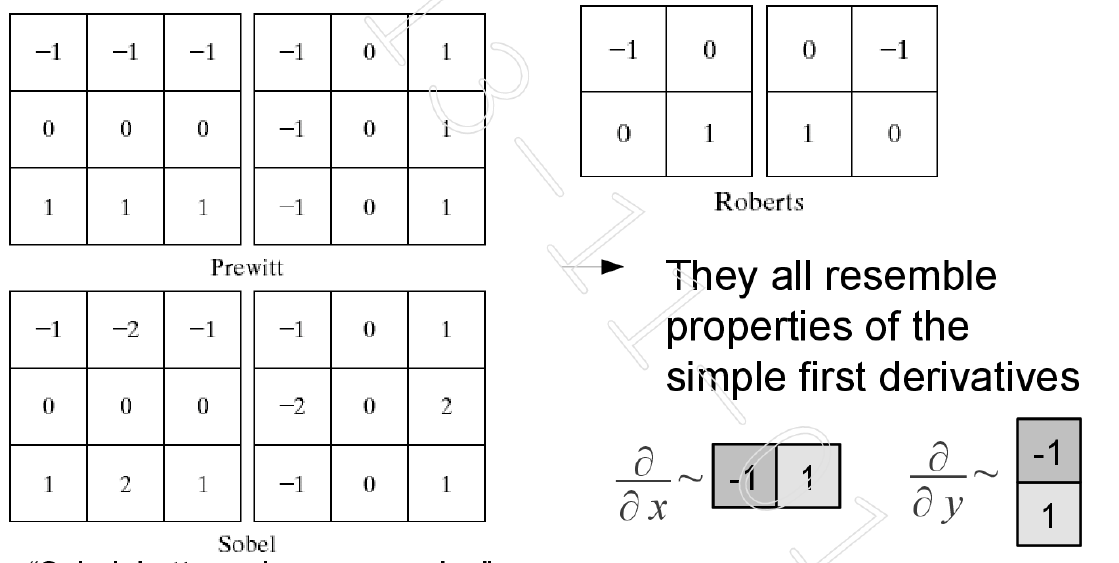
\includegraphics[width=\textwidth]{Bilder/edge_detection.png}
De sier at Sobel fjerner støy mer effektivt enn Prewitt.

Det er lett å konkludere at retningen på kantenene står normalt på gradientvektoren.

Det skal særdeles lite støy til før at de deriverte blir ubrukelige. Derfor vi smoother først.


Består gjerne av tre deler:
\begin{enumerate}
    \item Image smoothing (støy kan få kanter "usynlige" for filtrene våre)
    \item Deteksjon av kandidatpunkter for kanter. Dette gjøres gjerne med et (high-pass-filter).
    \item Kantlokalisering
\end{enumerate}

\subsubsection{Laplacian of Gaussian}
Laplacian blir sjelden brukt alene, fordi den er for sensitiv for støy. Vi kan kombinere Laplacian med Gaussian slik at vi får begge deler samtidig. Et sammensatt filter (også kalt mexcan hat) ser da slik ut:
\\ 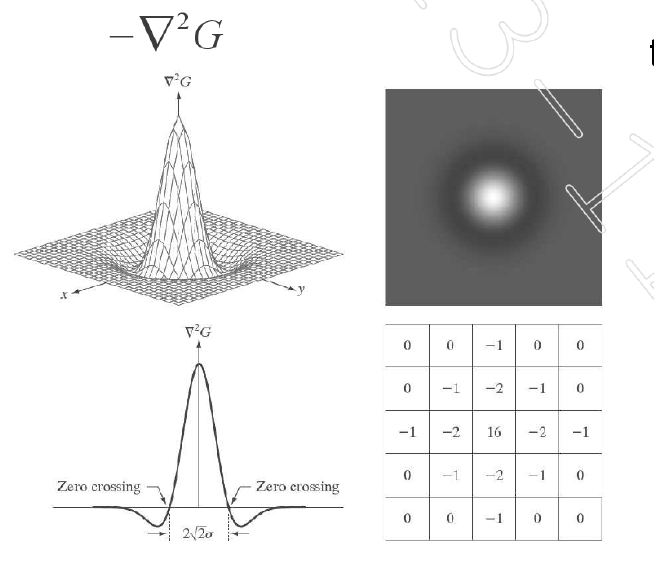
\includegraphics[width=\textwidth]{Bilder/mexican.PNG}

Marr-Hildreth-algoritmen ser da på et bilde som er filtrert med LoG-filteret og finner zero-crossings.
\\ 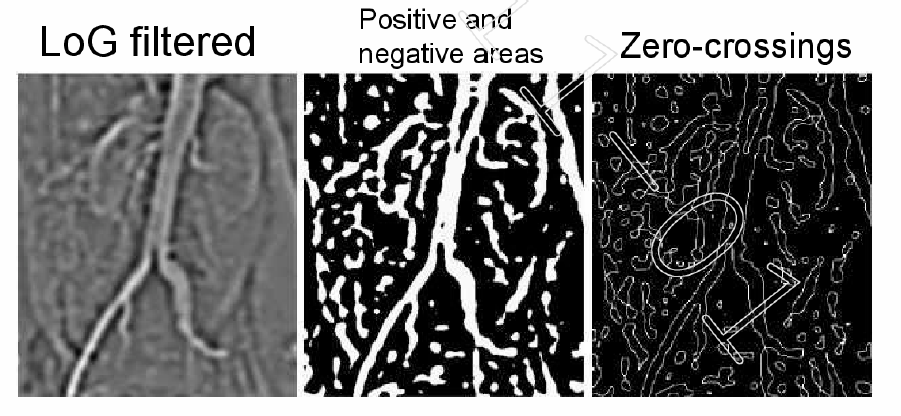
\includegraphics[width=\textwidth]{Bilder/log.png}

\subsubsection{Zero Crossing}
Gitt følgende matrise:
$$
    \begin{matrix}
        A & B & C \\
        D & p & D \\
        C & B & A
    \end{matrix}
$$
kan man sjekke om bokstav-parene har forskjellig fortegn. Har de det, har vi en zero crossing.

Har man en 2x2-matrise kans man sjekke om begge fortegn forekommer i matrisen.

\subsubsection{Canny edge detection}
Bruker LoG-filteret, og bruker to thresholds for å klassifisere svake og sterke kanter. Sterke kanter blir alltid med, svake kanter blir bare med dersom de er koblet til sterke kanter.

\subsection{Hough Transform}
Gjør om et linjestykke fra parametrene $m$ og $b$ til parametrene $r$ og $\Theta$.
\begin{equation}
    y = mx + b = -{cos(\Theta) \over sin(\Theta)}x + {r \over sin(\Theta)}
\end{equation}
Denne takler også vertikale linjer.

En linje vil i parameter-rommet $(r, \Theta)$ være et punkt. Hvis du da f.eks. har fire punkt, kan du tegne alle linjene som går igjennom et punkt i dette rommet. Hvert punkt vil da lage en linje i parameterrommet. Der alle møtes, er linjen som går igjennom alle fire punkt.

Transformen blir da:
\begin{enumerate}
    \item Gjør om til et binært bilde med feks canny edges
    \item Del opp parameterrommet i akkumulatorceller (satt til 0, mulighet for å økes)
    \item For hvet punkt i det binære bildet, øk akkumulatorcellene der parameterkurven passer igjennom.
    \item Lokale maksima i akkumulatormatrisen vil mest sannsynlig tilvare linjer i det binære bildet.
\end{enumerate}

\subsection{Corner detection}
Når vi detekterer hjørner, forventer vi en endring i intensitet uansett hvordan vi flytter oss (et kantfilter vil ikke endre seg om vi flytter det langs kanten). Vi bruker en matrise A som en \emph{structure tensor} og ser på egenverdiene til denne matrisen.

\begin{itemize}
    \item $\lambda_1 \approx 0$ og $\lambda_2 \approx 0$ gir en flat region.
    \item $\lambda_1 \approx 0$ og $\lambda_2 > 0$ gir en kantregion.
    \item $\lambda_1 > 0$ og $\lambda_2 > 0$ gir et hjørne.
\end{itemize}

\subsection{Morphological processing}
Når man er ferdig med segmentering, trenger man gjerne å jobbe litt mer med bildene. I bildebehandling bruker man matematisk morfologi som et verktøy for å ta ut bildekomponenter som er nyttige for beskrivelsen og representasjonen av en figur.

\subsection{Basic set operations}
Differansen til et sett er:
\begin{equation}
    A - B = \{w|w \in A, w \notin B \}
\end{equation}
Refleksjonen til et sett er:
\begin{equation}
    \hat B = \{w|\text{$w=-b$ for $b \in B$}\}
\end{equation}
For symmetriske sett er $B=\hat B$.

\subsection{Structuring element}
For morfologiske operasjoner definerer man et struktureringselement sammen med en referansepiksel.
\\ 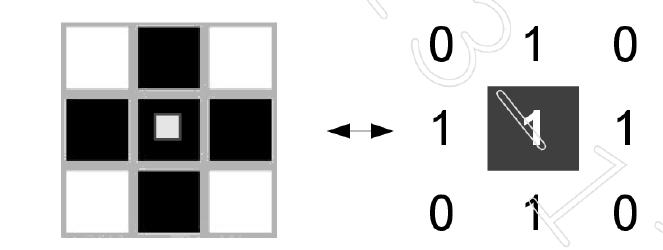
\includegraphics[width=\textwidth]{Bilder/se.png}

\subsection{Erosion $f \ominus  s$}
Dette er en "fit"-operasjon, her må masken passe fullstendig. Regionene vil bli mindre. Man farger "output pixel" dersom hele masken passer fullstendig. Matematisk definisjon

\begin{equation}
    A \ominus  B = \{ z|(B)_z \subseteq A \}
\end{equation}
Husk at dette ikke er en lineær operasjon, siden den bruker set-operasjoner.

\subsection{Diation $f \oplus  s$}
Dette er en "hit"-operasjon, det holder at masken treffer på ett element. Man farger "output pixel" dersom masken treffer på ett element.

\begin{equation}
    A \oplus  B = \{ z|(\hat B)_z \cap A \neq \emptyset \}
\end{equation}
Ikke lineær operasjon.

\subsection{Dualitet}
Erosion of A by B is the compliment of the dilation of $A^C$ by $\hat B$.
\begin{equation}
    (A \ominus  B)^C = A^C \oplus \hat B
\end{equation}

\begin{equation}
    (A \oplus  B)^C = A^C \ominus \hat B
\end{equation}

\subsection{Closing $f \bullet  s$}
Dilation først, så erosion. Navnet kommer av at hvis man er inni et element med "hull", vil denne operasjonen tette hullene.

\subsection{Opening $f \circ  s$}
Erosion først, så dilation. Fjerner små objekter. Kan også brukes for å finne figurer i et bilde, fordi den tar med seg figurer hvor struktureringselementet passer.

\subsection{Opening og closing}
Disse operasjonene er idempotent. Det betyr at hvis man utfører de en gang til på et bilde, får du samme resultat.

\subsection{Hit-and-Miss Transform}
\begin{equation}
    A \otimes  B= (A \ominus  B_1) \cap  (A^C \ominus  B_2)
\end{equation}
Her er $B_1$ masken for forgrunnspiksler og $B_2$ masken for bakgrunnspiksler.

\subsection{Boundary Extraction}
Det eroderte bildet blir trukket fra orginalbildet. Man sitter da igjen med en kant.
\begin{equation}
    \Gamma (A) = A - (A \ominus  B)
\end{equation}

\subsection{Tilknyttede komponenter}
Begynn med en seeding piksel $x_0$ og regn ut $x_k$ iterativt ved å kjøre dilate til $x_k= x_{k-1}$.

\subsection{Filling holes}
Fyll bakgrunnen, og regn det som er igjen som deler av objektet.

\subsection{Thinning}
Det kan være ønskelig å sitte igjen med tynne linjer for å enklere kunne klassifisere. Dette kan man blant annet gjøre ved å bruke en sekvens av forskjellige hit-and-miss masker.
\\ 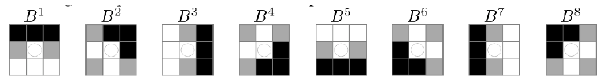
\includegraphics[width=\textwidth]{Bilder/hnm.png}

\subsection{Watershed Segmentation}
Se på dette som nedslagsfelt til regn. En regndråpe på hver enkelt piksel vil renne ned til et lokalt minimum (tenk på bildet som en tredimensjonal struktur der z-aksen er høyden). Grensen mellom disse nedslagsfeltene vil tegnes i bildet og vil være separate regioner.

\subsubsection{Distance Transform}
Watershed kan være nyttig med distansetransformasjon av et binært bilde. Hver enkel piksel regner ut sin distanse til nærmeste bakgrunnselement. Hvis man inverserer denne transformen, vil områder som er lengst unna bakgrunnen være lokale minima, og vil kunne brukes av watershed. Spesielt nyttig er dette for å skille elementer fra hverandre.
\\ 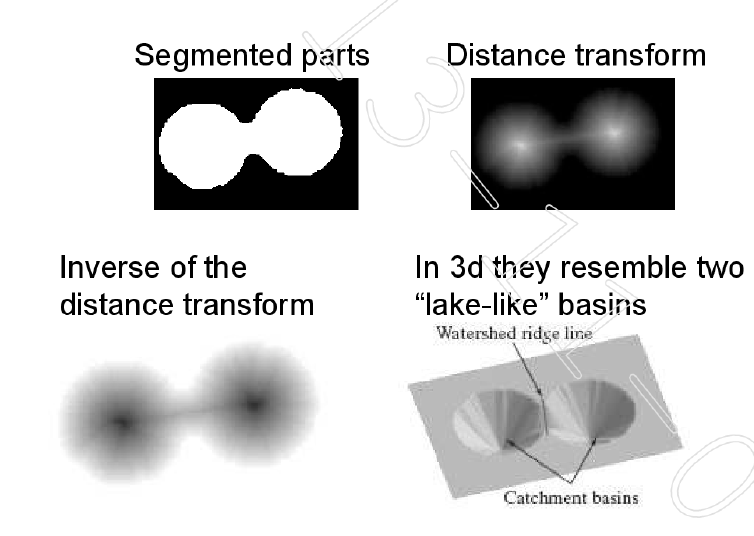
\includegraphics[width=\textwidth]{Bilder/watershed.png}

\subsection{Shape Description}
Ønsker man å gjenkjenne en enkel figur, kan man regne ut en éndimensjonal figur ved hjelp av et punkt (gjerne i midten) og distansen ut til kantene. Du vil få gjenkjennbare signaturer.
\\ 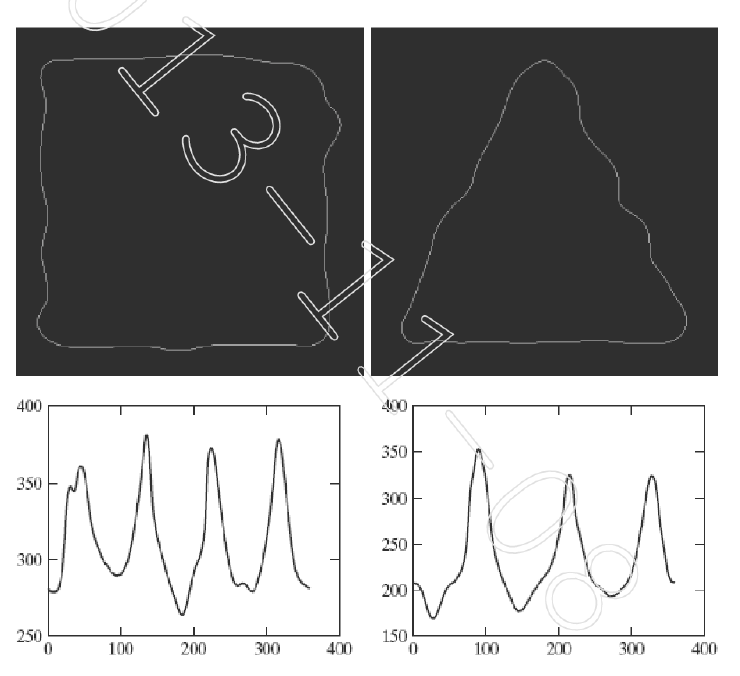
\includegraphics[width=\textwidth]{Bilder/sign.png}
\subsection{Annet småplukk}

\subsubsection{Region}
En region er et sett med piksler som er knyttet sammen. Hver eneste piksel tilfredsstiller kravene for å være en del av regionen.


















































